\documentclass{article}
\usepackage[utf8]{inputenc}
\usepackage[T1]{fontenc}
\usepackage{color}
\usepackage{geometry}
\geometry{a4paper, left=1.8cm, right=2.0cm, top=1.1cm, bottom=2.2cm}
\usepackage{amssymb}
\usepackage{amsmath}
\usepackage{graphicx}
\usepackage[english]{babel}

\title{Group project - Nonlinear model}
\author{Daniel Gilgen, David Lehnen, Matthias Roggo, Fabio Marti}
\date{\today}

\begin{document}
\maketitle
\parindent 0pt
\linespread{1.2} \selectfont
\numberwithin{equation}{section}
\parskip 10pt

Consider the following mechanical system

\begin{center}
%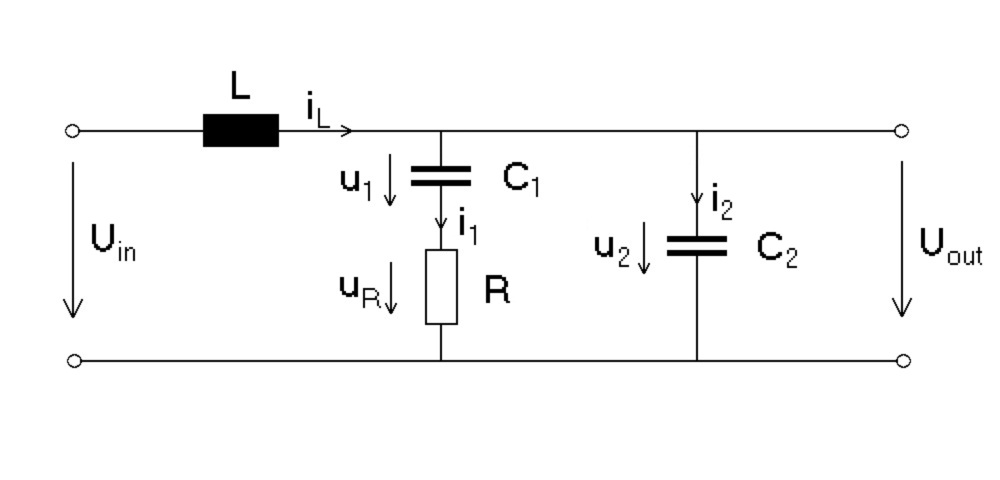
\includegraphics[width=14cm]{circuit_diagram}
\end{center}


We assume now that the wheel doesn't have a mass and that mass \(m_1\) has a moment of inertia of \(J_1 = c_1 m_1\) and mass \(m_2\) has \(J_2 = c_2 m_2\) with respect to the wheel's hub. Furthermore we are assuming that the force of the damper is given by \(F_b = b \cdot \Delta z\). Using Newton's laws we obtain the equations

\[
\begin{aligned}
m_3 \ddot{z}\quad &=\quad m_3 g + k (\varphi R - z) + b (\dot{\varphi}R - \dot{z}) \\\\
(J_1 + J_2)\ddot{\varphi}\quad &=\quad \tau + gd\cos(\varphi)(m_2 - m_1) + k(z - \varphi R) + b(\dot{z} - \dot{\varphi}R)
\end{aligned}
\]

By definig the states \(x_1 = z\), \(x_2 = \dot{z}\), \(x_3 = \varphi\) and \(x_4 = \dot{\varphi}\), the input \(u = \tau\) and the output \(y = \dot{\varphi}\) we find the following differential equations

\[
\begin{aligned}
\dot{x}_1\quad &=\quad x_2\\\\
\dot{x}_2\quad &=\quad g + \frac{k}{m_3} (x_3 R - x_1) + \frac{b}{m_3} (x_4 R - x_2)\\\\
\dot{x}_3\quad &=\quad x_4\\\\
\dot{x}_4\quad &=\quad \frac{1}{c_1 m_1 + c_2 m_2} \left( u + gd\cos(x_3)(m_2 - m_1) + k(x_1 - x_3 R) + b(x_2 - x_4R) \right) \\\\
y\quad &=\quad x_4
\end{aligned}
\]

In a next step we transform our continuous time system into a discrete time system. We use a simple Euler step for this task

\[\dot{x} \approx \frac{x_{k+1} - x_k}{T}\]

where \(T\) is the sampling period. The discrete system's equations now look as follows

\[
\begin{aligned}
x_{1,k+1}\quad &=\quad x_{1,k} + T\cdot  x_{2,k} \\\\
x_{2,k+1}\quad &=\quad x_{2,k} + T\cdot \left( g + \frac{k}{m_3} (x_{3,k} R - x_{1,k}) + \frac{b}{m_3} (x_{4,k} R - x_{2,k}) \right) \\\\
x_{3,k+1}\quad &=\quad x_{3,k} + T\cdot x_{4,k} \\\\
x_{4,k+1}\quad &=\quad x_{4,k} + T\cdot \left( \frac{1}{c_1 m_1 + c_2 m_2} \left( \tau + gd\cos(x_{3,k})(m_2 - m_1) + k(x_{1,k} - x_{3,k} R) + b(x_{2,k} - x_{4,k}R) \right) \right) \\\\
y_k\quad &=\quad x_{4,k}
\end{aligned}
\]



\end{document}